\documentclass{anotherarticlestyle}
\usepackage{multirow}
\title{A Very Impressive Report}
\author{A. Tilla$^{1,*}$, A. Menta$^{1, \dagger}$}
\correspondence{tucorreo@yahoo.cat, $^{\dagger}$otrocorreo@outlook.org}
\affiliations{Universidad de La Laguna}
\header{Report}

\leftheader{Subject Report Belongs To}
\rightheader{Master degree ni Astrophysics}

\setlength{\headheight}{13.6pt}
\addtolength{\topmargin}{-1.6pt}





\begin{document}

\maketitle

\begin{strip}
    \begin{abstract}
        {\small We did this and that and found this other thing and it was all very good and correct.}
    \end{abstract}
\end{strip}

\section{Introduction}
Galaxies, composed of stars, gas, and dust bound by gravitational forces, present complex patterns in their surface brightness distributions. Since its inception, the Hubble sequence \citep{hubble1982realm} has served as a cornerstone for classifying these celestial objects based on their morphological features, such as their elliptical shape, spiral arms or the presence of stellar central bars. However, the Hubble sequence has its limitations, including subjectivity in classification, a focus on superficial features rather than underlying physical properties, and a dependency on factors such as the galaxy's orientation (inclination) and the wavelength range of observations, rendering it incomplete for comprehensive astrophysical analysis.

Building on this foundation, photometric analysis of galaxy images has emerged as a robust tool for morphological analysis and classification, overcoming many limitations of the traditional classification.
%as each galaxy has a different superficial brightness distribution which depends in part on its morphology. 
As early as in the late 1980s, specialized software programs were developed to quantitatively analyze the brightness distribution of galaxies \citep{stetson1987daophot, mighell1989accurate}, allowing for a more objective and detailed understanding of their structure, which in turn shades light into their formation and evolution. Modern solutions like Imfit, developed by \citet{erwin2015imfit}, are contributing to the advancement of this field. Written in C++ and being open-source software, Imfit sets itself apart from older programs by going beyond radial profile analysis and being specifically designed for fitting 2D models into observational galaxy data images.
% It sets itself apart from older programs by going beyond radial profile analysis, incorporating Levenberg–Marquardt (L-M) gradient-search method for optimal fitting \citep{levenberg1944method, marquardt1963algorithm}. 



\begin{figure}
  \centering
  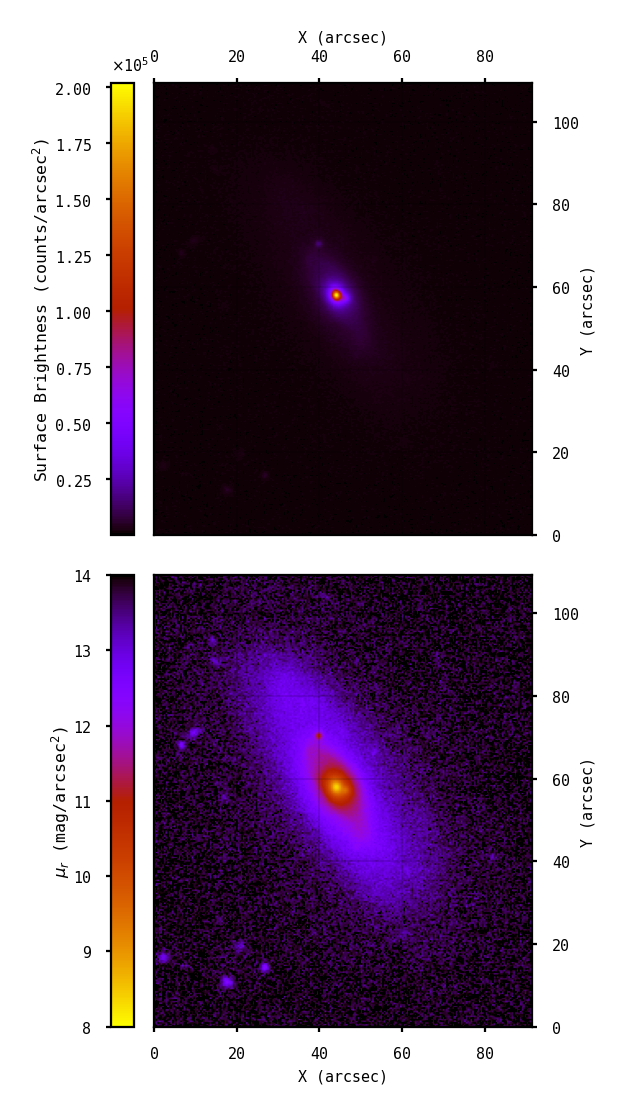
\includegraphics[width=1\columnwidth]{images/flux_mag_plot.png}  % adjust the width as you like
\caption{\small Near infrared ('i' band) image of UGC09629, observed on 2002-05-09 at Apache Point Observatory as a part of the Sloan Digital Sky Survey (SDSS). Exposure time was 53.91 seconds. (Top) surface brightness in counts per arcsecond$^2$. (Bottom) the same field in magnitudes per arcsecond squared. Axes of both figures are in arcseconds.}
  \label{fig:1}
\end{figure}

%

In the present study, we use Imfit to perform a photometric decomposition of the galaxy UGC09629 (see Figure \ref{fig:1}), situated in the constellation of Boötes, located in the northern celestial hemisphere as viewed from Earth at a declination of approximately 52 degrees north of the celestial equator. It is an Sa-type spiral galaxy with an estimated diameter of 60.31 kpc and it is receding from our Solar System at a velocity of approximately 7822 km s$^{-1}$ \citep{ned}. Based on the current (Planck satellite) value of the Hubble constant ($H_0=67.8 \ \text{km} \ \text{s}^{-1} \text{Mpc}^{-1}$) \citep{aghanim2020planck}, this translates to an estimated heliocentric distance of around $115.3$ Mpc. 

In the following sections, we construct and analyse three distinct 2D photometric models for the optimal fitting to discern UGC09629 morphological features. Isophotal profile analysis is also included. Finally, we discuss the limitations of our models and some potential improvements of our approach.




%¿Añadir expresión de Hubble?
%¿Imagen de la galaxia?


\section{Methodology}

\vspace{0.1in}
{\noindent\large\textcolor{ullpurple}{\textit{2.1 Image file analysis}}}
\vspace{0.1in}

A \texttt{fits} file containing photometric data of the galaxy UGC09629 with a pixel-length resolution $R_{\text{px}} = 0.396$ arcsec/px was supplied for our analysis. The initial measurements were in Analog Digital Units (ADUs), which we converted to detector electron counts--or 'counts' for short--by multiplying them by the given CCD-dependent gain of $g=6.565$ counts/ADU. It's crucial to note that an average sky value of 221.61 ADUs had already been subtracted from the initial image; an adjustment that has to be accounted for in subsequent analyses. Additionally, the readout noise specified for the dataset was 5.76 counts. A calibration constant, $Z_\text{cal}=-23.60$, was also provided for the conversion from surface brightness to magnitudes. We recall that surface brightness is measured in this context in counts/arcsec$^2$ and that its expression in magnitudes is 
\begin{equation}
    \mu_{r}=-2,5\log_{10}(I[\text{counts}/\text{arcsec}^2]) +Z_{cal}^\prime \ ,
\end{equation}
where $Z_{\text{cal}}^\prime = \lvert Z_\text{cal} \rvert + 5log_{10}(R_{\text{px}})$ is the new magnitude calibration constant for surface brightness.\footnote{That is, $Z_{cal}^\prime$ is the calibration constant for the magnitude derived from the flux in counts/arcsec$^2$, as opposed to the calibration constant $Z_\text{cal}$ for the magnitude derived from a flux in counts/pixel} All results below will be provided in surface brightness magnitudes. It is important to mention that the original \texttt{fits} file contains negative values due to sky subtraction, which could pose issues when converting to the magnitude scale. To address this, we have shifted the original data so that the most negative value becomes zero, ensuring that every pixel now has a positive-definite flux value. This adjustment has a negligible impact on the subsequent analysis, as the flux within the galaxy far exceeds the small offset value.

Additionally, we simulate the convolution of an ideal 'true' image with a point-spread function (PSF) to account for atmospheric and telescope-induced distortions. We use a Moffat function to model the PSF, a common approach for its ability to capture the wing-like structure in the star profiles. For our PSF, we set parameters with a FWHM of 1.25136 arcsec and a Beta of 3.59, generating a 51x51 pixel image in FITS format to ensure sufficient sampling. Imfit efficiently handles the PSF normalization and convolution process \citep{erwin2015imfit}.

\vspace{0.1in}
{\noindent\large\textcolor{ullpurple}{\textit{2.2 Fitting 2D models}}}
\vspace{0.1in}


Analysis of surface brightness data, as shown in Figure 1, reveals distinct structural components: mainly, a central bulge and an encompassing disk. Additionally, when examining the galaxy in magnitude scale, a localized luminosity peak near the galaxy's center is apparent. We hypothetise that this feature could potentially be another galaxy merging with UGC09629 or a foreground star along our line of sight. This lump will be relevant in the selection of 2D photometric models used in subsequent analyses.

To model these observations, we adhere to common practice by employing a S\'{e}rsic profile for the bulge and an exponential function for the disk. An additional S\'{e}rsic profile will be considered in one model for the localized luminosity peak. The S\'{e}rsic profile can be expressed as 
\begin{equation}
    I(R)=I_{e}\exp\left(-b_{n}\left[\left(\frac{R}{R_{e}}\right)^{1/n}-1\right]\right) \ ,
    \label{eq:sers}
\end{equation}
where \( I_{e} \) is the effective surface brightness, \( R_{e} \) the effective radius, \( n \) the S\'{e}rsic index, and \( b_{n} \) a normalization constant to ensure that \( R_{e} \) encloses half of the light within the bulge. On the other hand, the exponential profile for the disk is given by 
\begin{equation}
    I(R)=I_{0}\exp\left(-\frac{R}{h}\right) \ ,
    \label{eq:exp}
\end{equation}
where \( I_{0} \) is the central intensity and \( h \) is the disk scale length. Though Eqns. (\ref{eq:sers},\ref{eq:exp}) describe one-dimensional profiles, it's crucial to note that these equations define elliptical isophotes when ellipticity and angle are specified in our 2D model.

% It is suggested to use an exponential function to model the disk and a Sérsic for the bulb, we can also use another Sérsic for the lump. 
% \begin{enumerate}
%     \item Sérsic profile: Empirically derived by \citet{sersic1963influence}: \begin{equation}
%         I(R)=I_{e}\exp(-b_{n}[(\frac{R}{R_{e}})^{\frac{1}{n}})-1])
%     \end{equation} 
%     Where \(I_{e}\) is the effective surface brightness, \(R_{e}\) the effective radius and n the Sérsic index, and \(b_{n}\) the function to assure \(R_{e}\) contains half of the light. 
%     \\ In magnitudes:
%     \begin{equation}
%         \mu (R)=\mu_{e}+\frac{2.5b_{n}}{ln(10)}((R/R_{e})^{1/n}-1)
%     \end{equation}
%     \item Exponential profile: Proposed by \citet{freeman1970disks} to describe stellar discs:
%     \begin{equation}
%         I(R)=I_{0}exp(-r/h)
%     \end{equation}
%     In magnitudes:
%     \begin{equation}
%         \mu (R)=\mu_{0}+\frac{2,5}{ln(10)}\frac{R}{h}
%     \end{equation}
%     Where \(I_{0}\) is the central intensity and \(h\) is the disc scale length. 
% \end{enumerate}


% Actually, in this work we develop 3 different models. First, we incorporate both an exponential and a Sérsic model, supplemented with elliptical isophote profile analysis. The second model consists of a Sérsic and a exponential model for the bulb and another Sérsic model for the lump. The last one is also a exponential and a Sérsic model for our galaxy but we use a customized ad hoc mask. Among these models we will explain which one is better.


Accompanying the galaxy image, a mask was also provided to exclude specific regions from the fitting procedure (see Panel a) in Figure \ref{fig:3}). The mask primarily targets the outermost regions of the image and bright points corresponding to stars, effectively omitting them from the fit. Notably, the mask does not obscure the localized luminosity peak near the galaxy's center.

Considering our preliminary visual inspection of our galaxy and the provided mask, we developed three distinct models to capture the structural features of UGC09629. 
\begin{itemize}
    \item \textit{Sérsic$+$Exponential}. We combine an exponential function for the disk and a S\'{e}rsic profile for the bulge. We use the original provided mask for the fitting process. 
    \item \textit{Sérsic$+$Exponential \& Sérsic (lump)}. We use a S\'{e}rsic profile for both the bulge and the localized luminosity peak near the galaxy's center, in addition to an exponential model for the disk. Original mask is used.
    \item \textit{Sérsic$+$Exponential with new mask}. We combine an exponential function for the disk and a S\'{e}rsic profile for the bulge. We use an alternative customized ``\textit{ad hoc}'' mask to refine the fit.
\end{itemize}
% Subsequent sections will detail the comparative efficacy of these models in capturing the photometric properties of the galaxy.

% Once the functions are decided we use Imfit \citep{erwin2015imfit} to find the best fit. Imfit allows for the specification of a composite 2D surface-brightness model. These models are then fitted to the observed data through nonlinear minimization techniques to achieve optimal fitting statistics.

Once the models to be fitted are determined  we use Imfit's non-linear minimization techniques to optimize model parameters. We opt for the Levenberg--Marquardt (L-M) gradient-search algorithm for its robust performance \citep{levenberg1944method, marquardt1963algorithm}. The primary objective of this optimization
is to minimize the Gaussian-based \(\chi^2\) statistic, defined as:

\[
\chi^2 = \sum_{i=0}^{N} \frac{z_i}{\sigma^2_i} \left(I_{d,i} - I_{m,i}\right)^2
\]

Here, \(I_{d,i}\) represents the observed data pixels, \(I_{m,i}\) the model data pixels. \(\sigma_i^2\) is the Gaussian error of the data pixel, and $z_i$ is a boolean factor accounting for the provided mask. This \(\chi^2\) statistic serves as our main metric for quantifying and comparing the quality of the fit across different models.

In addition to the $\chi^2$ statistic, we also use the Akaike Information Criterion (AIC) \citep{akaike1998information} and the Bayesian Information Criterion (BIC) \citep{schwarz1978estimating} for quantifying the quality of the fit. Both metrics incorporate a penalty term for the number of parameters in the model and aim to be minimized, helping to prevent overfitting.

Regarding the customized mask. To construct it, we began with the residual image generated from subtracting our Sersic+Exponential model fit from the observed galaxy image. This residual image highlights the disparities between the model and actual data. We selected pixel values that were in the top 1 percentile of brightness on the magnitude scale. These outliers usually correspond to individual stars or other luminous components that are not part of the galaxy itself, although we understand they could also be due to intrinsic morphological components of the galaxy not accounted by an overly simplistic model. By isolating these points, we created a mask that can be used to exclude these extraneous components from further analysis, thereby refining our model's accuracy.

\vspace{0.1in}
{\noindent\large\textcolor{ullpurple}{\textit{2.3 Photometric decomposition routines}}}
\vspace{0.1in}

For galaxy model fitting we leveraged both the native Imfit program and its Python wrapper, pyImfit, which is publicly available on GitHub \url{https://github.com/perwin/pyimfit}.\footnote{Last consulted on 10/02/2023}. We also made extensive use of the Photutils package for isophote profiling, as described in \citep{jedrzejewski1987ccd}. The Python wrapper for Imfit was used for its enhanced modularity, allowing us to create a dedicated repository for our codebase, which can be found at \url{https://github.com/pererossello/galactic_photofit}, and accessible for further detail on our methods and full reproducibility of our results.
 % We develop 2D images of the model and the residual, also we plot 1D radial profiles of the position angle, the \(\mu_{r}\) magnitude and the ellipticity.
% We can derive other physical quantities: the apparent magnitude and the relation \(B/T=\frac{L_{bulb}}{L_total}\) and \(D/T=\frac{L_{disk}}{L_{total}}\). Imfit will automatically provide these quantities using the command \textit{makeimage bestfit\_parameters\_imfit.dat --save-fluxes fluxes.dat --zero-point=23.597900 --nrows=231 --ncols=276.} \\
% After successfully finding the best fit, Imfit will give back a model in FITS format and the parameters of the functions with the best fitting. The model in FITS format has the superficial brightness in \(counts/pixel^{2}\) and the distance in pixels, to make the necessary conversions we use the fact that 1 pixel is equivalent to 0,396 arcsec. \\ 
% To obtain the distance \(R\) in \(kpc\) we know that 
% \begin{equation}
%     R(kpc)=D(kpc)tan(\frac{0,369r [px]}{3600 [arcsec]})
% \end{equation}
% Where \(D\) the distance of the galaxy. We can compute \(D\) using the Hubble Law \(D=\frac{zc}{H_{0}}\) where \(z\) is the redshift and \(H_{0}\) the Hubble constant. We already know that \(D=115.3 Mpc\). 
% To convert our intensity from the model [counts/\(pixel^{2}\)] we have to multiply by the gain, because our model is in ADU, and the scale from \(pixels^{2}\) to \(arcsec^{2}\). Then, we can estimate the superficial brightness \(\mu _{r} (mag/arcsec^{2})\) using the relation:
% \begin{equation}
%     \mu_{r}=-2,5log_{10}(I(R)) +Z_{cal}+5log_{10}(0,396)
% \end{equation}
% Where \(Z_{cal}\) is the calibration magnitude in absolute value. \\
% Remember that with \textit{makeimage} we estimate the apparent magnitude and the \(B/T\), \(R/T\) ratios. Therefore, we can get the absolute magnitude:
% \begin{equation}
%     M=m-5log_{10}(\frac{d [pc]}{10})
% \end{equation}
% The image of the galaxy UGC 09629 was captured using the 'i' band, which is a specific photometric band in the near-infrared part of the electromagnetic spectrum. In the Sloan Digital Sky Survey (SDSS), the 'i' band centers roughly around 7671 Ångströms. This observation was carried out on May 9, 2002, at the SDSS's dedicated 2.5m telescope located at Apache Point Observatory in Southern New Mexico. The exposure time for the image was approximately 53.9 seconds. ¿En la parte de la introducción?
% We also used the Python wrapper for Imfit, which is publicly available at the following GitHub repository: \url{https://github.com/perwin/pyimfit}.\footnote{Last consulted on 10/02/2023}. In our python code we use the isophote fitting method used in photutils package: \citep{jedrzejewski1987ccd}.\\

\section{Results}
\lipsum[1]

\begin{table}[!htb]
  \centering
  \resizebox{0.485\textwidth}{!}{%  % This line changes the table width
    \begin{tabular}{|c|l|c|c|}
      \hline
      \multicolumn{4}{|c|}{\textbf{Parametros}}                                    \\
      \hline
      \textbf{Functions} & \textbf{Parameters} & \textbf{Results} & \textbf{Error} \\
      \hline
      \multirow{5}{*}{Coffee}
                         & Roast Level         & \(Dark\)         & \(N/A\)        \\
                         & Caffeine (mg)       & \(90\)           & \(5\)          \\
                         & Volume (ml)         & \(350\)          & \(10\)         \\
                         & Temperature (ºC)    & \(80\)           & \(2\)          \\
                         & Milk Volume (ml)    & \(50\)           & \(5\)          \\
      \hline
      \multirow{4}{*}{Pizza}
                         & Diameter (cm)       & \(30\)           & \(1\)          \\
                         & Toppings            & \(Pepperoni\)    & \(N/A\)        \\
                         & Calories            & \(2000\)         & \(100\)        \\
                         & Slices              & \(8\)            & \(0\)          \\
      \hline
    \end{tabular}
  }
  \caption{An example table with one column width.}
\end{table}

\lipsum[1]

\begin{table*}[h!]
  \centering
  \begin{tabular}{|c|l|c|c|}
    \hline
    \multicolumn{4}{|c|}{\textbf{The Ultimate Caffeine + Junk Food Smackdown}}                                     \\
    \hline
    \textbf{Beverages/Snacks} & \textbf{Parameters}         & \textbf{Epic Results} & \textbf{Confidence Interval} \\
    \hline
    \multirow{5}{*}{Espresso Extravaganza}
                              & Brew Time (seconds)         & \(30\)                & \(1\)                        \\
                              & Jitters Factor (\%)         & \(120\)               & \(±5\)                       \\
                              & Hipster Approval Rating     & \(100\)               & \(N/A\)                      \\
                              & Ideal Sipping Temp (ºC)     & \(85\)                & \(2\)                        \\
                              & Existential Crises Averted  & \(7\)                 & \(±1\)                       \\
    \hline
    \multirow{5}{*}{Donut Delirium}
                              & Sugar Coma Threshold (mins) & \(15\)                & \(3\)                        \\
                              & Sprinkle Count              & \(Hundreds, maybe?\)  & \(Don't make me count!\)     \\
                              & Glaze Viscosity (cP)        & \(500\)               & \(50\)                       \\
                              & 'Dunkability' Score         & \(9.5/10\)            & \(±0.2\)                     \\
                              & Eaten By (team members)     & \(Everyone\)          & \(N/A\)                      \\
    \hline
  \end{tabular}
  \caption{A stupid full-width table generated with GPT.}
\end{table*}

\lipsum[1-5]

\lipsum[1-4]

\begin{figure*}[h!]
  \centering
  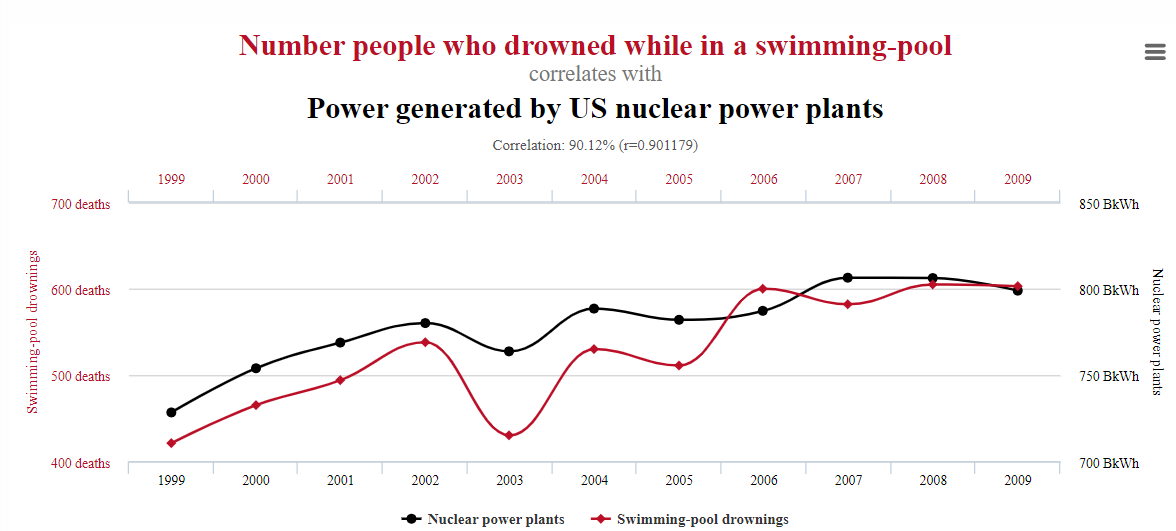
\includegraphics[width=\textwidth]{images/correlation.png}
  \caption{An example of figure spanning two columns.}
  \label{fig:your_label}
\end{figure*}


\lipsum[1-4]

\section{Conclusions}
% Overall, we can conclude that our results have been satisfactory. We developed three models that fit our galaxy with \(\chi _{red} ^{2}\) close to 1, being the Sérsic+exp & Sérsic (lump) our best model with \(\chi _{red} ^{2}=2.5\). Because \(\chi _{red} ^{2}\) is not 1, our model can be improved. Furthermore, if we see our residual map there are some galaxy arms that our model cannot take into account: the exponential function treats the disk as a continuum. 
% \\The primary objective of this endeavor was to learn how to perform a photometric decomposition, a goal that has been confidently and effectively realized.

% In summary, our investigation met its primary goal of unraveling the complexities of photometric decomposition, yielding encouraging results. Among the models we tested, the hybrid S\'{e}rsic plus Exponential and S\'{e}rsic (lump) configuration stood out with a reduced \( \chi_{\text{red}}^{2} \) of 2.5. While not precisely at the ideal value of 1, this measure indicates a reasonable fit. Moreover, the higher \( \chi_{\text{red}}^{2} \) can be attributed to certain structural complexities in the galaxy, such as spiral arms, not adequately handled by our mathematical framework. It's worth mentioning the customized mask, which managed to lower the \( \chi_{\text{red}}^{2} \) to 1.82, suggesting an even better fit. However, this improvement must be taken with a grain of caution: the mask was constructed in an ad-hoc manner by post-selecting the most prominent residuals, effectively giving it an advantage in minimizing \( \chi_{\text{red}}^{2} \). This 'tailoring' likely contributes to overfitting, a suspicion substantiated by the increase in AIC and BIC values. Hence, while the mask yields the best \( \chi_{\text{red}}^{2} \), its very nature tempers enthusiasm regarding its true predictive power.


In summary, our investigation met its primary goal of unraveling the complexities of photometric decomposition, yielding consistent results. Among the models we tested, the hybrid S\'{e}rsic plus Exponential and S\'{e}rsic (lump) configuration stood out with a reduced \( \chi_{\text{red}}^{2} \) of 2.5. While not precisely at the ideal value of 1, this measure indicates a reasonable fit. Moreover, the higher \( \chi_{\text{red}}^{2} \) can be attributed to certain structural complexities in the galaxy, such as spiral arms, not adequately handled by our mathematical framework. It's worth mentioning the customized mask, which managed to lower the \( \chi_{\text{red}}^{2} \) to 1.82, suggesting an even better fit. However, this improvement must be taken with caution: the mask was constructed in an ad-hoc manner by post-selecting the most prominent residuals, effectively giving it an advantage in minimizing \( \chi_{\text{red}}^{2} \). Future work could consider more intricate models specifically tailored for capturing the effects of spiral arms to improve the fit.


% \section*{Data Availability Statement}
% The data supporting the findings of this study, along with the code and methodologies employed, are publicly available on GitHub. For complete details on our methods and to fully reproduce our results, interested parties can refer to the following repository: \url{https://github.com/pererossello/galactic_photofit}.

\newpage
\pagebreak

\section*{References}
\bibliographystyle{plainnat}
\bibliography{refs}



% Comment if you don't want Supplementary Tables or Figures

\onecolumn
\newpage
\pagebreak
\section*{Supplementary Tables}


\begin{table}[!htb]
    \renewcommand{\thetable}{S1}
    \centering
    \begin{tabular}{|c|l|c|c|}
        \hline
        \multicolumn{4}{|c|}{\textbf{Global Parameters}} \\
        \hline
        \multicolumn{4}{|c|}{\(X_{0} = 111.66 \pm 0.0\), \(Y_{0} = 147.07 \pm 0.0\)} \\
        \hline
        \multicolumn{4}{|c|}{\(\chi^{2}_{\text{red}} = 2.5\), \(\text{AIC} = 37641.39\), \(\text{BIC} = 37778.48\)} \\
        \hline
        \textbf{Functions} & \textbf{Parameters} & \textbf{Results} & \textbf{Error} \\
        \hline
        \multirow{5}{*}{Sérsic} 
        & PA (º) & \(21.94\) & \(0.28\) \\
        & Ell & \(0.21\) & \(0.0\) \\
        & \(n\) & \(1.63\) & \(0.0\) \\
        & \(I_{e}\) (counts/\(px^{2}\)) & \(700\) & \(0.0\) \\
        & \(R_{e}\) (px) & \(6.12\) & \(0.01\) \\
        \hline
        \multirow{4}{*}{Exponential}
        & PA (º) & \(29.36\) & \(0.06\) \\
        & Ell & \(0.66\) & \(0.0\) \\
        & \(I_{0}\) (counts/\(px^{2}\)) & \(289.28\) & \(1.41\) \\
        & \(h\) (px) & \(30.98\) & \(0.1\) \\
        \hline
        \multirow{5}{*}{Sérsic (Lump)}
        & \(X_{1}\) & \(117.13\) & \(0.02\) \\
        & \(Y_{1}\) & \(145.22\) & \(0.02\) \\
        & PA (º) & \(68.32\) & \(1.39\) \\
        & Ell & \(0.25\) & \(0.01\) \\
        & \(n\) & \(1.53\) & \(0.04\) \\
        & \(I_{e}\) (counts/\(px^{2}\)) & \(166.4\) & \(5.27\) \\
        & \(R_{e}\) (px) & \(4.2\) & \(0.09\) \\
        \hline
    \end{tabular}
     \caption{Parameters for the Exponential + Sérsic \& Sérsic (Lump) Model}
    \label{tab:my_label}
\end{table}

\begin{table}[!htb]
    \renewcommand{\thetable}{S2}
    \centering
    \begin{tabular}{|c|l|c|c|}
        \hline
        \multicolumn{4}{|c|}{\textbf{Exponential + Sérsic \& Sérsic (Lump)}} \\
        \hline
        \textbf{Component} & \textbf{m} & \textbf{M} & \textbf{B/T} \\
        \hline
        Bulb & \(9.8785\) & \(-25.43\) & \(0.32976\) \\
        \hline
        Disk & \(9.1650\) & \(-26.14\) & \(0.63618\) \\
        \hline
        Lump & \(12.3436\) & \(-22.97\) & \(0.03405\) \\
        \hline
    \end{tabular}
    \caption{Magnitudes and Bulge Disk Ratios for the Exponential + Sérsic \& Sérsic (Lump) Model. }
\end{table}


\newpage


\begin{table}[!htb]
    \renewcommand{\thetable}{S3}
    \centering
    \begin{tabular}{|c|l|c|c|}
        \hline
        \multicolumn{4}{|c|}{\textbf{Exponential + Sérsic with Customized Mask}} \\
        \hline
        \multicolumn{4}{|c|}{\(X_{0} = 111.9 \pm 0.0\), \(Y_{0} = 147.02 \pm 0.0\)} \\
        \hline
        \multicolumn{4}{|c|}{\(\chi_{\text{red}}^{2} = 1.82\), \(\text{AIC} = 114583.56\), \(\text{BIC} = 114683.14\)} \\
        \hline
        \textbf{Functions} & \textbf{Parameters} & \textbf{Results} & \textbf{Error} \\
        \hline
        \multirow{5}{*}{Sérsic}
        & PA (º) & \(32.08\) & \(0.23\) \\
        & Ell & \(0.21\) & \(0.0\) \\
        & \(n\) & \(1.44\) & \(0.01\) \\
        & \(I_{e}\) (counts/\(px^{2}\)) & \(795.28\) & \(4.1\) \\
        & \(R_{e}\) (px) & \(5.96\) & \(0.02\) \\
        \hline
        \multirow{4}{*}{Exponential}
        & PA (º) & \(29.43\) & \(0.06\) \\
        & Ell & \(0.64\) & \(0.0\) \\
        & \(I_{0}\) (counts/\(px^{2}\)) & \(300.06\) & \(1.64\) \\
        & \(h\) (px) & \(29.76\) & \(0.1\) \\
        \hline
    \end{tabular}
    \caption{Parameters for the Exponential + Sérsic Model with customized mask}
\end{table}

\begin{table}[!htb]
    \renewcommand{\thetable}{S4}
    \centering
    \begin{tabular}{|c|l|c|c|}
        \hline
        \multicolumn{4}{|c|}{\textbf{Exponential + Sérsic}} \\
      
        \multicolumn{4}{|c|}{\textbf{with ad hoc customised mask}} \\
        \hline
        \textbf{Component} & \textbf{m} & \textbf{M} & \textbf{B/T} \\
        \hline
        Bulb & \(9.8585\) & \(-25.45\) & \(0.34251\) \\
        \hline
        Disk & \(9.1505\) & \(-26.16\) & \(0.65749\) \\
        \hline
    \end{tabular}
    \caption{Magnitudes and Bulge Disk Ratios for the Exponential + Sérsic model with customised mask. }
\end{table}







% \begin{table}[!htb]
%     \centering
%     \begin{tabular}{|c|l|c|c|}
%         \hline
%         \multicolumn{4}{|c|}{\textbf{Exponential + Sérsic Model}} \\
%         \hline
%         \multicolumn{4}{|c|}{\(X_{0} = 111.98 \pm 0.00\), \(Y_{0} = 146.95 \pm 0.00\)} \\
%         \hline
%         \multicolumn{4}{|c|}{\(\chi^{2}_{\text{red}} = 3.38\), \(\text{AIC} = 50886.79\), \(\text{BIC} = 50970.57\)} \\
%         \hline
%         \textbf{Functions} & \textbf{Parameters} & \textbf{Results} & \textbf{Error} \\
%         \hline
%         \multirow{5}{*}{Sérsic} 
%         & PA (º) & \(39.88\) & \(0.22\) \\
%         & Ell & \(0.20\) & \(0.00\) \\
%         & \(n\) & \(1.37\) & \(0.01\) \\
%         & \(I_{e}\) (counts/\(px^{2}\)) & \(844.67\) & \(3.91\) \\
%         & \(R_{e}\) (px) & \(5.85\) & \(0.02\) \\
%         \hline
%         \multirow{4}{*}{Exponential}
%         & PA (º) & \(28.73\) & \(0.06\) \\
%         & Ell & \(0.65\) & \(0.00\) \\
%         & \(I_{0}\) (counts/\(px^{2}\)) & \(311.7\) & \(1.77\) \\
%         & \(h\) (px) & \(29.73\) & \(0.10\) \\
%         \hline
%     \end{tabular}
%     \caption{Parameters for the Exponential + Sérsic model}
% \end{table}


\twocolumn
\onecolumn
\newpage
\pagebreak
\section*{Supplementary Figures}
\begin{figure*}[h!]
\renewcommand{\thefigure}{S1}
  \centering
  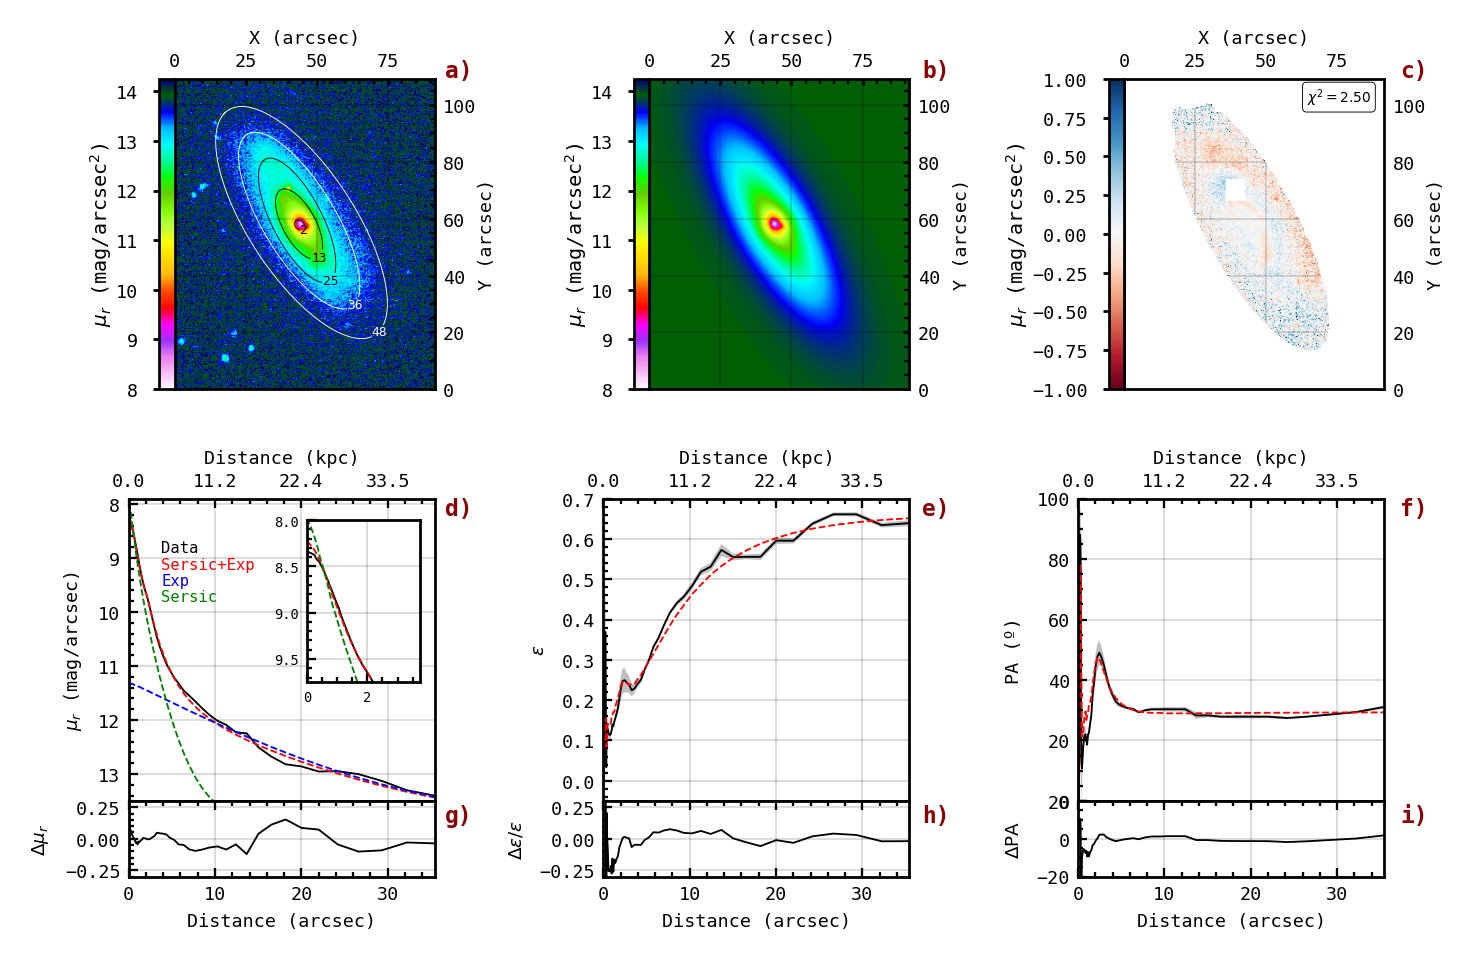
\includegraphics[width=\textwidth]{images/fit_sersic_exp_and_sersic_bump.png}
  \caption{Photometric fitting of UGC09629 incorporating an exponential and a Sérsic model for the galaxy and an additional Sérsic model for the luminous bulb near the center of the galaxy, supplemented with elliptical isophote profile analysis. The reduced $\chi^2$ for the overall fit was 2.50. Image description is the same as Figure 2 in the main text.}
  \label{fig:your_label}
\end{figure*}


\begin{figure*}[h!]
\renewcommand{\thefigure}{S2}
  \centering
  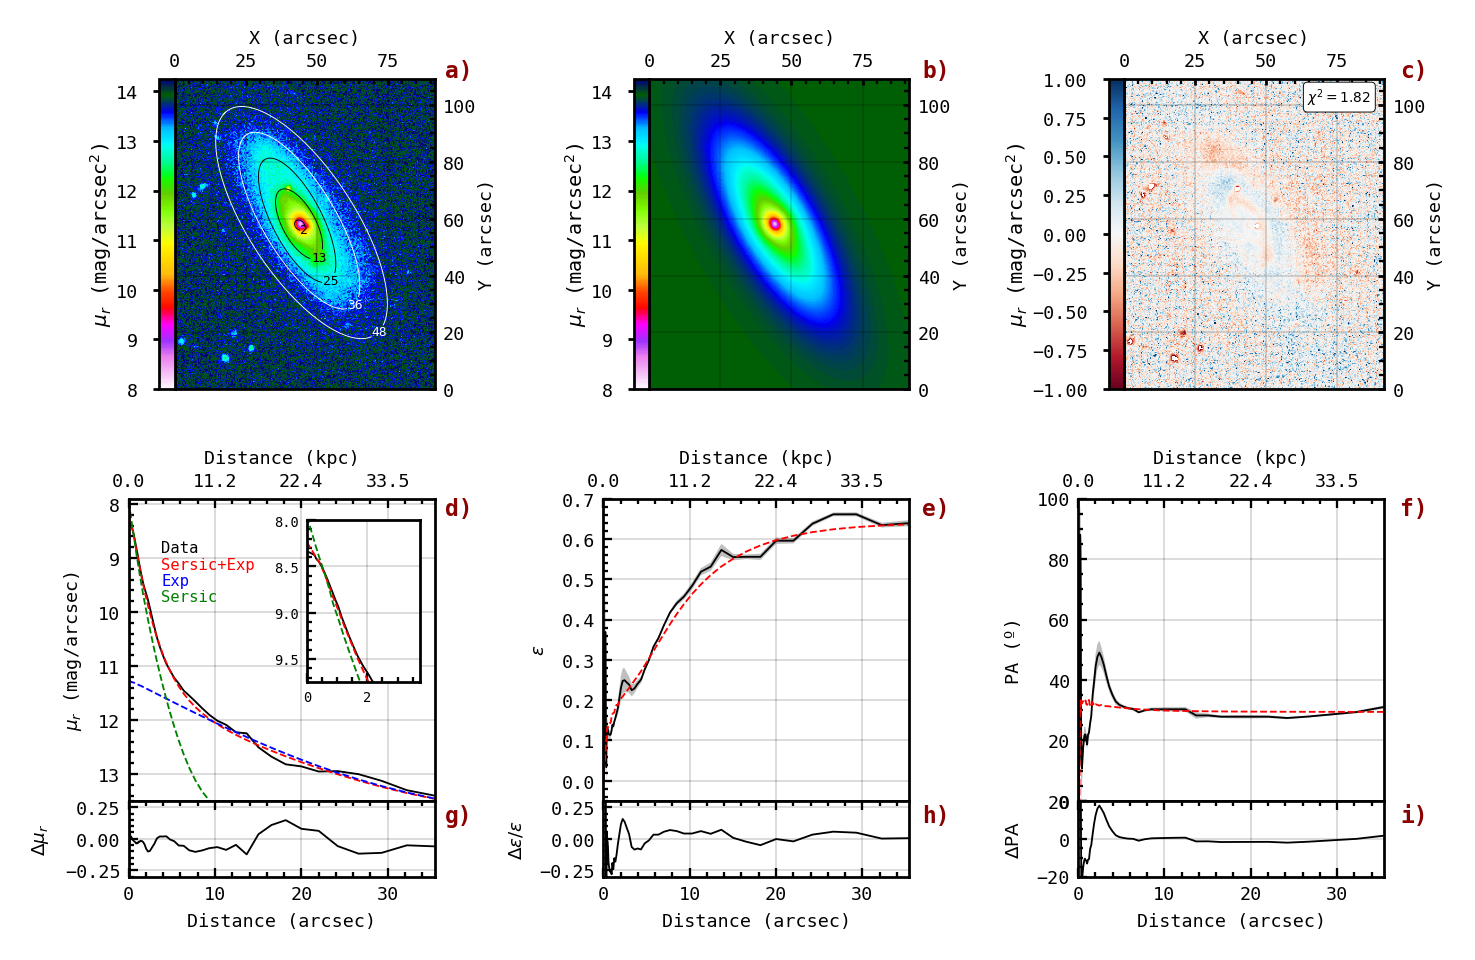
\includegraphics[width=\textwidth]{images/fit_sersic_exp_own_mask.png}
  \caption{Photometric fitting of UGC09629 incorporating an exponential and a Sérsic model for the galaxy and using a customized \textit{ad hoc} mask, supplemented with elliptical isophote profile analysis. The reduced $\chi^2$ for the overall fit was 1.82. Image description is the same as Figure 2 in the main text.}
  \label{fig:your_label}
\end{figure*}



\end{document}



% 

% \section{Methodology}

% 
\vspace{0.1in}
{\noindent\large\textcolor{ullpurple}{\textit{2.1 Image file analysis}}}
\vspace{0.1in}

A \texttt{fits} file containing photometric data of the galaxy UGC09629 with a pixel-length resolution $R_{\text{px}} = 0.396$ arcsec/px was supplied for our analysis. The initial measurements were in Analog Digital Units (ADUs), which we converted to detector electron counts--or 'counts' for short--by multiplying them by the given CCD-dependent gain of $g=6.565$ counts/ADU. It's crucial to note that an average sky value of 221.61 ADUs had already been subtracted from the initial image; an adjustment that has to be accounted for in subsequent analyses. Additionally, the readout noise specified for the dataset was 5.76 counts. A calibration constant, $Z_\text{cal}=-23.60$, was also provided for the conversion from surface brightness to magnitudes. We recall that surface brightness is measured in this context in counts/arcsec$^2$ and that its expression in magnitudes is 
\begin{equation}
    \mu_{r}=-2,5\log_{10}(I[\text{counts}/\text{arcsec}^2]) +Z_{cal}^\prime \ ,
\end{equation}
where $Z_{\text{cal}}^\prime = \lvert Z_\text{cal} \rvert + 5log_{10}(R_{\text{px}})$ is the new magnitude calibration constant for surface brightness.\footnote{That is, $Z_{cal}^\prime$ is the calibration constant for the magnitude derived from the flux in counts/arcsec$^2$, as opposed to the calibration constant $Z_\text{cal}$ for the magnitude derived from a flux in counts/pixel} All results below will be provided in surface brightness magnitudes. It is important to mention that the original \texttt{fits} file contains negative values due to sky subtraction, which could pose issues when converting to the magnitude scale. To address this, we have shifted the original data so that the most negative value becomes zero, ensuring that every pixel now has a positive-definite flux value. This adjustment has a negligible impact on the subsequent analysis, as the flux within the galaxy far exceeds the small offset value.

Additionally, we simulate the convolution of an ideal 'true' image with a point-spread function (PSF) to account for atmospheric and telescope-induced distortions. We use a Moffat function to model the PSF, a common approach for its ability to capture the wing-like structure in the star profiles. For our PSF, we set parameters with a FWHM of 1.25136 arcsec and a Beta of 3.59, generating a 51x51 pixel image in FITS format to ensure sufficient sampling. Imfit efficiently handles the PSF normalization and convolution process \citep{erwin2015imfit}.

\vspace{0.1in}
{\noindent\large\textcolor{ullpurple}{\textit{2.2 Fitting 2D models}}}
\vspace{0.1in}


Analysis of surface brightness data, as shown in Figure 1, reveals distinct structural components: mainly, a central bulge and an encompassing disk. Additionally, when examining the galaxy in magnitude scale, a localized luminosity peak near the galaxy's center is apparent. We hypothetise that this feature could potentially be another galaxy merging with UGC09629 or a foreground star along our line of sight. This lump will be relevant in the selection of 2D photometric models used in subsequent analyses.

To model these observations, we adhere to common practice by employing a S\'{e}rsic profile for the bulge and an exponential function for the disk. An additional S\'{e}rsic profile will be considered in one model for the localized luminosity peak. The S\'{e}rsic profile can be expressed as 
\begin{equation}
    I(R)=I_{e}\exp\left(-b_{n}\left[\left(\frac{R}{R_{e}}\right)^{1/n}-1\right]\right) \ ,
    \label{eq:sers}
\end{equation}
where \( I_{e} \) is the effective surface brightness, \( R_{e} \) the effective radius, \( n \) the S\'{e}rsic index, and \( b_{n} \) a normalization constant to ensure that \( R_{e} \) encloses half of the light within the bulge. On the other hand, the exponential profile for the disk is given by 
\begin{equation}
    I(R)=I_{0}\exp\left(-\frac{R}{h}\right) \ ,
    \label{eq:exp}
\end{equation}
where \( I_{0} \) is the central intensity and \( h \) is the disk scale length. Though Eqns. (\ref{eq:sers},\ref{eq:exp}) describe one-dimensional profiles, it's crucial to note that these equations define elliptical isophotes when ellipticity and angle are specified in our 2D model.

% It is suggested to use an exponential function to model the disk and a Sérsic for the bulb, we can also use another Sérsic for the lump. 
% \begin{enumerate}
%     \item Sérsic profile: Empirically derived by \citet{sersic1963influence}: \begin{equation}
%         I(R)=I_{e}\exp(-b_{n}[(\frac{R}{R_{e}})^{\frac{1}{n}})-1])
%     \end{equation} 
%     Where \(I_{e}\) is the effective surface brightness, \(R_{e}\) the effective radius and n the Sérsic index, and \(b_{n}\) the function to assure \(R_{e}\) contains half of the light. 
%     \\ In magnitudes:
%     \begin{equation}
%         \mu (R)=\mu_{e}+\frac{2.5b_{n}}{ln(10)}((R/R_{e})^{1/n}-1)
%     \end{equation}
%     \item Exponential profile: Proposed by \citet{freeman1970disks} to describe stellar discs:
%     \begin{equation}
%         I(R)=I_{0}exp(-r/h)
%     \end{equation}
%     In magnitudes:
%     \begin{equation}
%         \mu (R)=\mu_{0}+\frac{2,5}{ln(10)}\frac{R}{h}
%     \end{equation}
%     Where \(I_{0}\) is the central intensity and \(h\) is the disc scale length. 
% \end{enumerate}


% Actually, in this work we develop 3 different models. First, we incorporate both an exponential and a Sérsic model, supplemented with elliptical isophote profile analysis. The second model consists of a Sérsic and a exponential model for the bulb and another Sérsic model for the lump. The last one is also a exponential and a Sérsic model for our galaxy but we use a customized ad hoc mask. Among these models we will explain which one is better.


Accompanying the galaxy image, a mask was also provided to exclude specific regions from the fitting procedure (see Panel a) in Figure \ref{fig:3}). The mask primarily targets the outermost regions of the image and bright points corresponding to stars, effectively omitting them from the fit. Notably, the mask does not obscure the localized luminosity peak near the galaxy's center.

Considering our preliminary visual inspection of our galaxy and the provided mask, we developed three distinct models to capture the structural features of UGC09629. 
\begin{itemize}
    \item \textit{Sérsic$+$Exponential}. We combine an exponential function for the disk and a S\'{e}rsic profile for the bulge. We use the original provided mask for the fitting process. 
    \item \textit{Sérsic$+$Exponential \& Sérsic (lump)}. We use a S\'{e}rsic profile for both the bulge and the localized luminosity peak near the galaxy's center, in addition to an exponential model for the disk. Original mask is used.
    \item \textit{Sérsic$+$Exponential with new mask}. We combine an exponential function for the disk and a S\'{e}rsic profile for the bulge. We use an alternative customized ``\textit{ad hoc}'' mask to refine the fit.
\end{itemize}
% Subsequent sections will detail the comparative efficacy of these models in capturing the photometric properties of the galaxy.

% Once the functions are decided we use Imfit \citep{erwin2015imfit} to find the best fit. Imfit allows for the specification of a composite 2D surface-brightness model. These models are then fitted to the observed data through nonlinear minimization techniques to achieve optimal fitting statistics.

Once the models to be fitted are determined  we use Imfit's non-linear minimization techniques to optimize model parameters. We opt for the Levenberg--Marquardt (L-M) gradient-search algorithm for its robust performance \citep{levenberg1944method, marquardt1963algorithm}. The primary objective of this optimization
is to minimize the Gaussian-based \(\chi^2\) statistic, defined as:

\[
\chi^2 = \sum_{i=0}^{N} \frac{z_i}{\sigma^2_i} \left(I_{d,i} - I_{m,i}\right)^2
\]

Here, \(I_{d,i}\) represents the observed data pixels, \(I_{m,i}\) the model data pixels. \(\sigma_i^2\) is the Gaussian error of the data pixel, and $z_i$ is a boolean factor accounting for the provided mask. This \(\chi^2\) statistic serves as our main metric for quantifying and comparing the quality of the fit across different models.

In addition to the $\chi^2$ statistic, we also use the Akaike Information Criterion (AIC) \citep{akaike1998information} and the Bayesian Information Criterion (BIC) \citep{schwarz1978estimating} for quantifying the quality of the fit. Both metrics incorporate a penalty term for the number of parameters in the model and aim to be minimized, helping to prevent overfitting.

Regarding the customized mask. To construct it, we began with the residual image generated from subtracting our Sersic+Exponential model fit from the observed galaxy image. This residual image highlights the disparities between the model and actual data. We selected pixel values that were in the top 1 percentile of brightness on the magnitude scale. These outliers usually correspond to individual stars or other luminous components that are not part of the galaxy itself, although we understand they could also be due to intrinsic morphological components of the galaxy not accounted by an overly simplistic model. By isolating these points, we created a mask that can be used to exclude these extraneous components from further analysis, thereby refining our model's accuracy.

\vspace{0.1in}
{\noindent\large\textcolor{ullpurple}{\textit{2.3 Photometric decomposition routines}}}
\vspace{0.1in}

For galaxy model fitting we leveraged both the native Imfit program and its Python wrapper, pyImfit, which is publicly available on GitHub \url{https://github.com/perwin/pyimfit}.\footnote{Last consulted on 10/02/2023}. We also made extensive use of the Photutils package for isophote profiling, as described in \citep{jedrzejewski1987ccd}. The Python wrapper for Imfit was used for its enhanced modularity, allowing us to create a dedicated repository for our codebase, which can be found at \url{https://github.com/pererossello/galactic_photofit}, and accessible for further detail on our methods and full reproducibility of our results.
 % We develop 2D images of the model and the residual, also we plot 1D radial profiles of the position angle, the \(\mu_{r}\) magnitude and the ellipticity.
% We can derive other physical quantities: the apparent magnitude and the relation \(B/T=\frac{L_{bulb}}{L_total}\) and \(D/T=\frac{L_{disk}}{L_{total}}\). Imfit will automatically provide these quantities using the command \textit{makeimage bestfit\_parameters\_imfit.dat --save-fluxes fluxes.dat --zero-point=23.597900 --nrows=231 --ncols=276.} \\
% After successfully finding the best fit, Imfit will give back a model in FITS format and the parameters of the functions with the best fitting. The model in FITS format has the superficial brightness in \(counts/pixel^{2}\) and the distance in pixels, to make the necessary conversions we use the fact that 1 pixel is equivalent to 0,396 arcsec. \\ 
% To obtain the distance \(R\) in \(kpc\) we know that 
% \begin{equation}
%     R(kpc)=D(kpc)tan(\frac{0,369r [px]}{3600 [arcsec]})
% \end{equation}
% Where \(D\) the distance of the galaxy. We can compute \(D\) using the Hubble Law \(D=\frac{zc}{H_{0}}\) where \(z\) is the redshift and \(H_{0}\) the Hubble constant. We already know that \(D=115.3 Mpc\). 
% To convert our intensity from the model [counts/\(pixel^{2}\)] we have to multiply by the gain, because our model is in ADU, and the scale from \(pixels^{2}\) to \(arcsec^{2}\). Then, we can estimate the superficial brightness \(\mu _{r} (mag/arcsec^{2})\) using the relation:
% \begin{equation}
%     \mu_{r}=-2,5log_{10}(I(R)) +Z_{cal}+5log_{10}(0,396)
% \end{equation}
% Where \(Z_{cal}\) is the calibration magnitude in absolute value. \\
% Remember that with \textit{makeimage} we estimate the apparent magnitude and the \(B/T\), \(R/T\) ratios. Therefore, we can get the absolute magnitude:
% \begin{equation}
%     M=m-5log_{10}(\frac{d [pc]}{10})
% \end{equation}
% The image of the galaxy UGC 09629 was captured using the 'i' band, which is a specific photometric band in the near-infrared part of the electromagnetic spectrum. In the Sloan Digital Sky Survey (SDSS), the 'i' band centers roughly around 7671 Ångströms. This observation was carried out on May 9, 2002, at the SDSS's dedicated 2.5m telescope located at Apache Point Observatory in Southern New Mexico. The exposure time for the image was approximately 53.9 seconds. ¿En la parte de la introducción?
% We also used the Python wrapper for Imfit, which is publicly available at the following GitHub repository: \url{https://github.com/perwin/pyimfit}.\footnote{Last consulted on 10/02/2023}. In our python code we use the isophote fitting method used in photutils package: \citep{jedrzejewski1987ccd}.\\
% \section{Results and Discussion}
% The most straightforward model under consideration is the Exponential + Sérsic combination. Figure 1 and Tables 1-2 showcase the outcomes and corresponding fit parameters for this model. Results for the other two models have been relegated to the supplementary material for brevity. Specifically, Figure S1 and Tables S1-S2 pertain to the Exponential + Sérsic \& Sérsic (lump) model, while Figure S2 and Tables S3-S4 correspond to the Exponential + Sérsic model using a custom mask. A comparative analysis of all three models is illustrated in Figure 3.

% The parameters obtained for the different models are shown in the tables below. We also add another table for the Sérsic, exponential and Sérsic for the lump model that includes the apparent magnitude and the ratios B/T.
% The figures \ref{fig:3}, \ref{fig:enter-label}, \ref{fig:your_label} and \ref{tab:my_label} represent the best fit 2D image and residuals, also the 1D radial profiles with the best fit over plotted.

\begin{table}[!htb]
    \centering
    \begin{tabular}{|c|l|c|c|}
        \hline
        \multicolumn{4}{|c|}{\textbf{Exponential + Sérsic Model}} \\
        \hline
        \multicolumn{4}{|c|}{\(X_{0} = 111.98 \pm 0.00\), \(Y_{0} = 146.95 \pm 0.00\)} \\
        \hline
        \multicolumn{4}{|c|}{\(\chi^{2}_{\text{red}} = 3.38\), \(\text{AIC} = 50886.79\), \(\text{BIC} = 50970.57\)} \\
        \hline
        \textbf{Functions} & \textbf{Parameters} & \textbf{Results} & \textbf{Error} \\
        \hline
        \multirow{5}{*}{Sérsic} 
        & PA (º) & \(39.88\) & \(0.22\) \\
        & Ell & \(0.20\) & \(0.00\) \\
        & \(n\) & \(1.37\) & \(0.01\) \\
        & \(I_{e}\) (counts/\(px^{2}\)) & \(844.67\) & \(3.91\) \\
        & \(R_{e}\) (px) & \(5.85\) & \(0.02\) \\
        \hline
        \multirow{4}{*}{Exponential}
        & PA (º) & \(28.73\) & \(0.06\) \\
        & Ell & \(0.65\) & \(0.00\) \\
        & \(I_{0}\) (counts/\(px^{2}\)) & \(311.7\) & \(1.77\) \\
        & \(h\) (px) & \(29.73\) & \(0.10\) \\
        \hline
    \end{tabular}
    \caption{Parameters for the Exponential + Sérsic model}
\end{table}


\begin{table}[!htb]
    \centering
    \begin{tabular}{|c|l|c|c|}
        \hline
        \multicolumn{4}{|c|}{\textbf{Exponential + Sérsic \& Sérsic}} \\
        \hline
        \textbf{Component} & \textbf{m} & \textbf{M} & \textbf{B/T} \\
        \hline
        Bulb & \(9.8442\) & \(-25.46\) & \(0.34371\) \\
        \hline
        Disk & \(9.1420\) & \(-26.17\) & \(0.65629\) \\
        \hline
        Total & \(8.6952\) & \(-26.61\) & \(1.00000\) \\
        \hline
    \end{tabular}
    \caption{Magnitudes and Bulge Disk Ratios for the Exponential + Sérsic model. }
\end{table}


\begin{figure*}[h!]
  \centering
  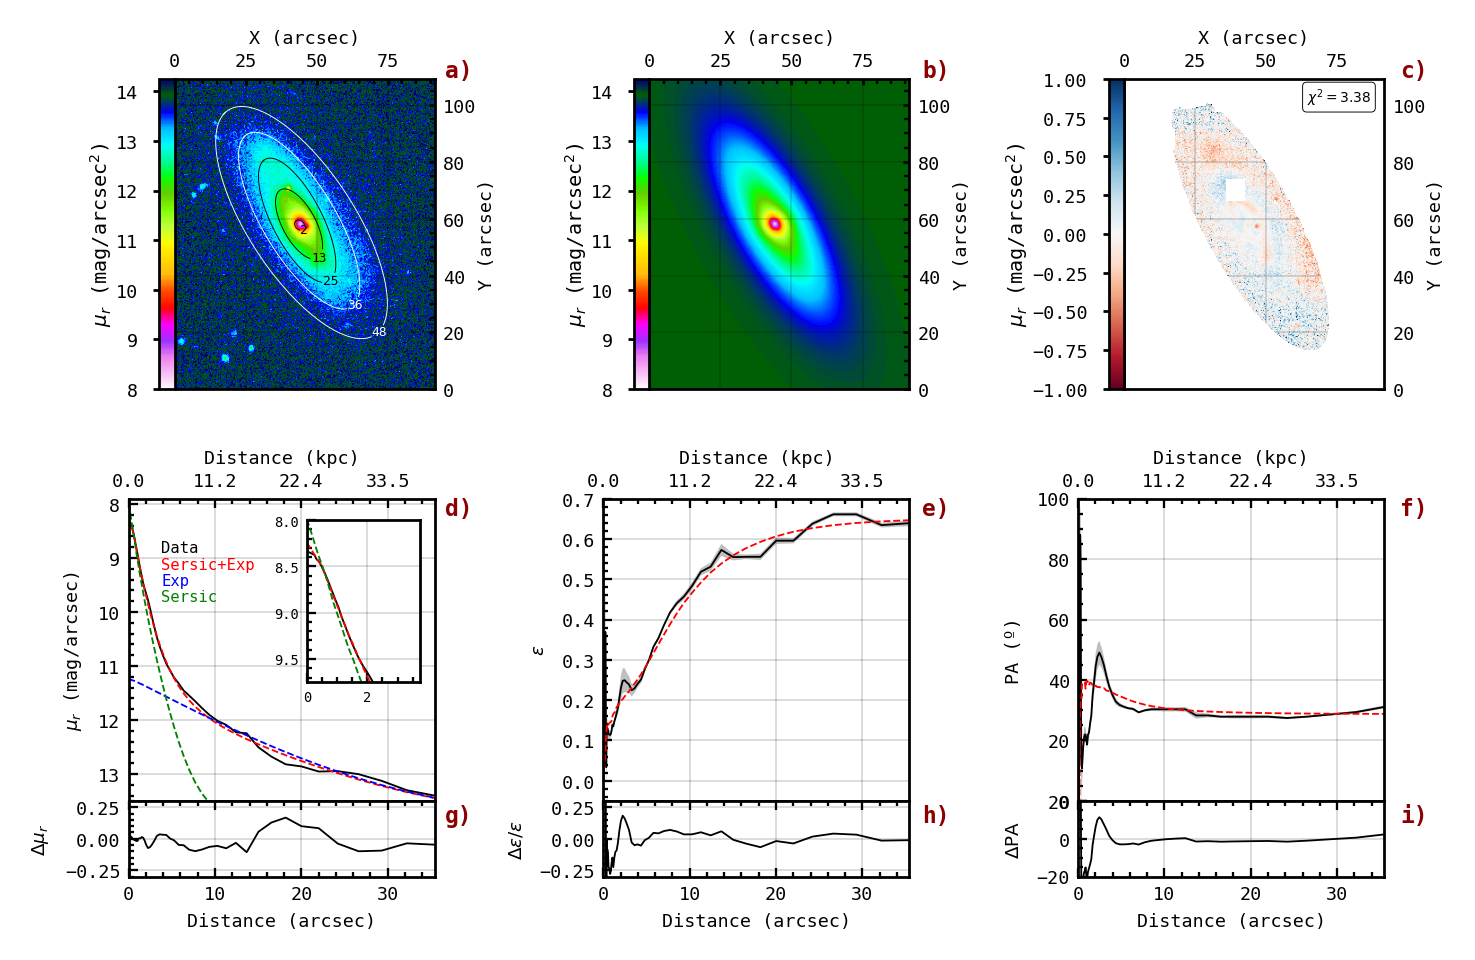
\includegraphics[width=\textwidth]{images/fit_sersic_exp.png}
\caption{\small Photometric fitting of UGC09629 incorporating both an exponential and a Sersic model, supplemented with elliptical isophote profile analysis. The reduced $\chi^2$ for the overall fit was 3.38. Panels (a, b, c) display images in units of magnitudes per arcsecond squared for the observed galaxy data (a), the best-fitting model (b), and the residual between them (c). On panel a) fitted elliptic isophotal lines are represented with their semi-major axis value in arcseconds. Panel (d) plots the isophotal profiles in arcseconds, comparing the observed data (black) with the full Sersic-exponential fit (red), the Sersic-only component (green), and the exponential-only component (blue). Panel (g) highlights the discrepancies between the observed isophotal profile and the best-fitting model. Panel (e) compares the ellipticity of isophotes between the observed data (black) and the best-fit model (red), with their differences detailed in panel (h). Lastly, panel (f) illustrates the orientation angle of the semi-major axis of elliptical isophotes relative to the Y-axis for both observed data (black) and best-fit model (red), and panel (i) quantifies their differences. Panels (d, e, f) feature gray shading --barely visible-- to indicate the error derived from the elliptical isophote fitting.}
  \label{fig:your_label}
\end{figure*}

The initial takeaway from our optimal fits across all models is a remarkable consistency in parameters, particularly concerning the ellipticities of the galactic bulge and the exponential disk. For instance, the ellipticity of the bulge hovers around \(0.21\), while the disk's ellipticity is approximately \(0.64\) for all models. This gradation in ellipticity is corroborated by the isophotal profile in Figure~2e for the Exponential + S\'{e}rsic model. Furthermore, all other parameters are similarly consistent across models, underscoring that all considered models predict analogous morphological features. Moreover, a shift in the position angle (PA) from the bulge to the disk is evident across the models, illustrating that the galaxy has an apparent skewness. The most notable disparity between models perhaps arises in the S\'{e}rsic \(I_{e}\) parameter when the model incorporates the lump, registering approximately a 12\% reduction compared to the other models. This observation aligns with the methodology for that model, where the stellar lump in the bulge is fitted separately, thereby excluding its influence on the primary galactic bulge parameter.

\begin{figure*}[h!]
  \centering
  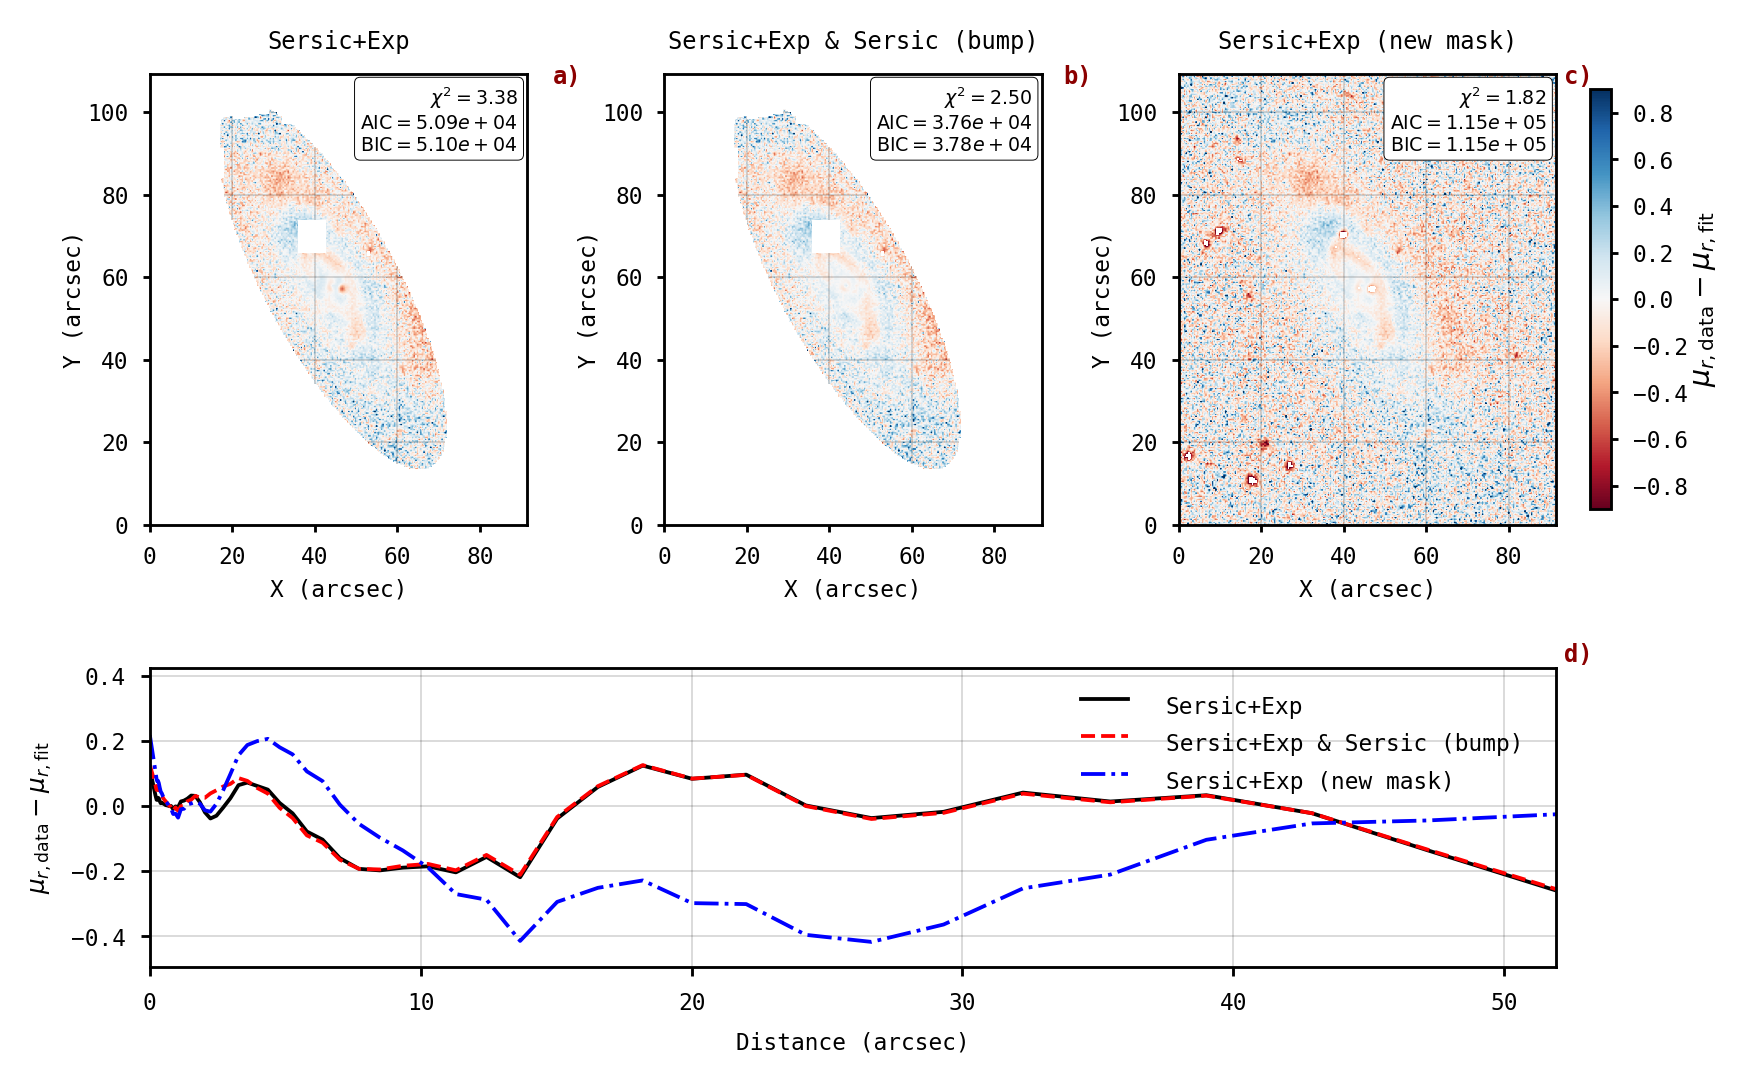
\includegraphics[width=\textwidth]{images/residual_comparison.png}
\caption{\small Comparative analysis of residuals and isophotal profile differences for three distinct fitting models: (a) Sersic-Exponential, (b) Sersic-Exponential with an additional Sersic component for the central bright region (bump), and (c) Sersic-Exponential with ad hoc masking. In panels (a, b, c), the residuals are displayed as the observational data subtracted from the respective best-fit models. The masks used for fitting are overlaid in white. Quality-of-fit metrics such as $\chi^2$, AIC, and BIC are also provided. Panel (d) showcases the discrepancies in the magnitude values for elliptical isophotal profiles between the observed data and each of the three fitting models.}
  \label{fig:3}
\end{figure*}

We measured a total integrated apparent magnitude of 8.7. Knowing that the distance is around $115.3$ Mpc\footnote{Based on the current (Planck satellite) value of the Hubble constant ($H_0=67.8 \ \text{km} \ \text{s}^{-1} \text{Mpc}^{-1}$) \citep{aghanim2020planck}}
this leads to a value of the absolute magnitude of -26.61. In the database \citep{ned} the galaxy UGC09629 has an apparent 
magnitude of \(10.806 \pm 0.031\) mag and an absolute magnitude of \(-24.57 \pm 0.5\) mag in the Near-IR H band. 
Although we measured in the `i' band, our results are similar, with a difference of 2.1 in magnitude. We can compare also the apparent magnitude of our galaxy with another Sa galaxies like NGC5351, which is \(56.10 \pm 3.93\) Mpc away. The apparent magnitude in the I band is \(10.90\) mag and the absolute magnitude \(-22.3\) mag, also similar to our results. 

The B/T ratios are also generally consistent across the different models, staying close to \(0.344\) for the bulge and \(0.656\) for the disk in the standard Exponential + Sérsic model. A slight variation is observed in the model that includes a lump, where the B/T ratio for the bulge drops to \(0.330\) and the disk's ratio increases to \(0.636\), with the lump taking up a ratio of \(0.034\). In the Exponential + Sérsic model using a customized mask, the B/T ratios are \(0.343\) for the bulge and \(0.657\) for the disk, showing virtually no departure from the standard model. The key divergence appears in the lump-inclusive model, a result that is again intuitive given the separate fit for the stellar lump in the bulge. The B/T ratios are consistent with the fact that our galaxy is Sa type, having a prominent bulb and a disk. 

In the standard Exponential + Sérsic model, the reduced \(\chi^{2}\) is \(3.38\), suggesting a somewhat poor fit given that a value closer to 1 would be ideal. The AIC and BIC values are \(50886.79\) and \(50970.57\), respectively. When we compare these metrics with the model that incorporates a Sérsic lump, the reduced \(\chi^{2}\) drops to \(2.5\), indicating a somewhat better fit. The AIC and BIC also show improvements, dropping to \(37641.39\) and \(37778.48\), respectively. For the Exponential + Sérsic model with a customized mask, the reduced \(\chi^{2}\) drops further to \(1.82\), nearing the ideal value of 1, yet the AIC and BIC increase to \(114583.56\) and \(114683.14\), which could be an indication overfitting. Given these metrics, one could argue that the lump-inclusive model performs better in terms of fit and overfitting trade-offs, although the customized mask seems to provide the best \(\chi^{2}\) value. 

Despite an extensive and automated search for optimal initial guesses to achieve the best fits, the \(\chi^{2}\) values could not be further reduced. This limitation is likely due to the presence of spiral arms in the galaxy, which our current models are not equipped to capture accurately. These spiral arms can be partially discerned in the residual plots shown in Figure 3. Furthermore, a consultation of external databases confirms that the galaxy belongs to the Sa type in the Hubble classification \citep{ned}, further corroborating the hypothesis that the inability to minimize \(\chi^{2}\) may be due to the complexity introduced by the spiral arms.




% \section{Conclusions}

% % Overall, we can conclude that our results have been satisfactory. We developed three models that fit our galaxy with \(\chi _{red} ^{2}\) close to 1, being the Sérsic+exp & Sérsic (lump) our best model with \(\chi _{red} ^{2}=2.5\). Because \(\chi _{red} ^{2}\) is not 1, our model can be improved. Furthermore, if we see our residual map there are some galaxy arms that our model cannot take into account: the exponential function treats the disk as a continuum. 
% \\The primary objective of this endeavor was to learn how to perform a photometric decomposition, a goal that has been confidently and effectively realized.

% In summary, our investigation met its primary goal of unraveling the complexities of photometric decomposition, yielding encouraging results. Among the models we tested, the hybrid S\'{e}rsic plus Exponential and S\'{e}rsic (lump) configuration stood out with a reduced \( \chi_{\text{red}}^{2} \) of 2.5. While not precisely at the ideal value of 1, this measure indicates a reasonable fit. Moreover, the higher \( \chi_{\text{red}}^{2} \) can be attributed to certain structural complexities in the galaxy, such as spiral arms, not adequately handled by our mathematical framework. It's worth mentioning the customized mask, which managed to lower the \( \chi_{\text{red}}^{2} \) to 1.82, suggesting an even better fit. However, this improvement must be taken with a grain of caution: the mask was constructed in an ad-hoc manner by post-selecting the most prominent residuals, effectively giving it an advantage in minimizing \( \chi_{\text{red}}^{2} \). This 'tailoring' likely contributes to overfitting, a suspicion substantiated by the increase in AIC and BIC values. Hence, while the mask yields the best \( \chi_{\text{red}}^{2} \), its very nature tempers enthusiasm regarding its true predictive power.


In summary, our investigation met its primary goal of unraveling the complexities of photometric decomposition, yielding consistent results. Among the models we tested, the hybrid S\'{e}rsic plus Exponential and S\'{e}rsic (lump) configuration stood out with a reduced \( \chi_{\text{red}}^{2} \) of 2.5. While not precisely at the ideal value of 1, this measure indicates a reasonable fit. Moreover, the higher \( \chi_{\text{red}}^{2} \) can be attributed to certain structural complexities in the galaxy, such as spiral arms, not adequately handled by our mathematical framework. It's worth mentioning the customized mask, which managed to lower the \( \chi_{\text{red}}^{2} \) to 1.82, suggesting an even better fit. However, this improvement must be taken with caution: the mask was constructed in an ad-hoc manner by post-selecting the most prominent residuals, effectively giving it an advantage in minimizing \( \chi_{\text{red}}^{2} \). Future work could consider more intricate models specifically tailored for capturing the effects of spiral arms to improve the fit.


% \section*{Data Availability Statement}
% The data supporting the findings of this study, along with the code and methodologies employed, are publicly available on GitHub. For complete details on our methods and to fully reproduce our results, interested parties can refer to the following repository: \url{https://github.com/pererossello/galactic_photofit}.





% \onecolumn
% \newpage
% \pagebreak
% \section*{Supplementary Tables}
% 

\begin{table}[!htb]
    \renewcommand{\thetable}{S1}
    \centering
    \begin{tabular}{|c|l|c|c|}
        \hline
        \multicolumn{4}{|c|}{\textbf{Global Parameters}} \\
        \hline
        \multicolumn{4}{|c|}{\(X_{0} = 111.66 \pm 0.0\), \(Y_{0} = 147.07 \pm 0.0\)} \\
        \hline
        \multicolumn{4}{|c|}{\(\chi^{2}_{\text{red}} = 2.5\), \(\text{AIC} = 37641.39\), \(\text{BIC} = 37778.48\)} \\
        \hline
        \textbf{Functions} & \textbf{Parameters} & \textbf{Results} & \textbf{Error} \\
        \hline
        \multirow{5}{*}{Sérsic} 
        & PA (º) & \(21.94\) & \(0.28\) \\
        & Ell & \(0.21\) & \(0.0\) \\
        & \(n\) & \(1.63\) & \(0.0\) \\
        & \(I_{e}\) (counts/\(px^{2}\)) & \(700\) & \(0.0\) \\
        & \(R_{e}\) (px) & \(6.12\) & \(0.01\) \\
        \hline
        \multirow{4}{*}{Exponential}
        & PA (º) & \(29.36\) & \(0.06\) \\
        & Ell & \(0.66\) & \(0.0\) \\
        & \(I_{0}\) (counts/\(px^{2}\)) & \(289.28\) & \(1.41\) \\
        & \(h\) (px) & \(30.98\) & \(0.1\) \\
        \hline
        \multirow{5}{*}{Sérsic (Lump)}
        & \(X_{1}\) & \(117.13\) & \(0.02\) \\
        & \(Y_{1}\) & \(145.22\) & \(0.02\) \\
        & PA (º) & \(68.32\) & \(1.39\) \\
        & Ell & \(0.25\) & \(0.01\) \\
        & \(n\) & \(1.53\) & \(0.04\) \\
        & \(I_{e}\) (counts/\(px^{2}\)) & \(166.4\) & \(5.27\) \\
        & \(R_{e}\) (px) & \(4.2\) & \(0.09\) \\
        \hline
    \end{tabular}
     \caption{Parameters for the Exponential + Sérsic \& Sérsic (Lump) Model}
    \label{tab:my_label}
\end{table}

\begin{table}[!htb]
    \renewcommand{\thetable}{S2}
    \centering
    \begin{tabular}{|c|l|c|c|}
        \hline
        \multicolumn{4}{|c|}{\textbf{Exponential + Sérsic \& Sérsic (Lump)}} \\
        \hline
        \textbf{Component} & \textbf{m} & \textbf{M} & \textbf{B/T} \\
        \hline
        Bulb & \(9.8785\) & \(-25.43\) & \(0.32976\) \\
        \hline
        Disk & \(9.1650\) & \(-26.14\) & \(0.63618\) \\
        \hline
        Lump & \(12.3436\) & \(-22.97\) & \(0.03405\) \\
        \hline
    \end{tabular}
    \caption{Magnitudes and Bulge Disk Ratios for the Exponential + Sérsic \& Sérsic (Lump) Model. }
\end{table}


\newpage


\begin{table}[!htb]
    \renewcommand{\thetable}{S3}
    \centering
    \begin{tabular}{|c|l|c|c|}
        \hline
        \multicolumn{4}{|c|}{\textbf{Exponential + Sérsic with Customized Mask}} \\
        \hline
        \multicolumn{4}{|c|}{\(X_{0} = 111.9 \pm 0.0\), \(Y_{0} = 147.02 \pm 0.0\)} \\
        \hline
        \multicolumn{4}{|c|}{\(\chi_{\text{red}}^{2} = 1.82\), \(\text{AIC} = 114583.56\), \(\text{BIC} = 114683.14\)} \\
        \hline
        \textbf{Functions} & \textbf{Parameters} & \textbf{Results} & \textbf{Error} \\
        \hline
        \multirow{5}{*}{Sérsic}
        & PA (º) & \(32.08\) & \(0.23\) \\
        & Ell & \(0.21\) & \(0.0\) \\
        & \(n\) & \(1.44\) & \(0.01\) \\
        & \(I_{e}\) (counts/\(px^{2}\)) & \(795.28\) & \(4.1\) \\
        & \(R_{e}\) (px) & \(5.96\) & \(0.02\) \\
        \hline
        \multirow{4}{*}{Exponential}
        & PA (º) & \(29.43\) & \(0.06\) \\
        & Ell & \(0.64\) & \(0.0\) \\
        & \(I_{0}\) (counts/\(px^{2}\)) & \(300.06\) & \(1.64\) \\
        & \(h\) (px) & \(29.76\) & \(0.1\) \\
        \hline
    \end{tabular}
    \caption{Parameters for the Exponential + Sérsic Model with customized mask}
\end{table}

\begin{table}[!htb]
    \renewcommand{\thetable}{S4}
    \centering
    \begin{tabular}{|c|l|c|c|}
        \hline
        \multicolumn{4}{|c|}{\textbf{Exponential + Sérsic}} \\
      
        \multicolumn{4}{|c|}{\textbf{with ad hoc customised mask}} \\
        \hline
        \textbf{Component} & \textbf{m} & \textbf{M} & \textbf{B/T} \\
        \hline
        Bulb & \(9.8585\) & \(-25.45\) & \(0.34251\) \\
        \hline
        Disk & \(9.1505\) & \(-26.16\) & \(0.65749\) \\
        \hline
    \end{tabular}
    \caption{Magnitudes and Bulge Disk Ratios for the Exponential + Sérsic model with customised mask. }
\end{table}







% \begin{table}[!htb]
%     \centering
%     \begin{tabular}{|c|l|c|c|}
%         \hline
%         \multicolumn{4}{|c|}{\textbf{Exponential + Sérsic Model}} \\
%         \hline
%         \multicolumn{4}{|c|}{\(X_{0} = 111.98 \pm 0.00\), \(Y_{0} = 146.95 \pm 0.00\)} \\
%         \hline
%         \multicolumn{4}{|c|}{\(\chi^{2}_{\text{red}} = 3.38\), \(\text{AIC} = 50886.79\), \(\text{BIC} = 50970.57\)} \\
%         \hline
%         \textbf{Functions} & \textbf{Parameters} & \textbf{Results} & \textbf{Error} \\
%         \hline
%         \multirow{5}{*}{Sérsic} 
%         & PA (º) & \(39.88\) & \(0.22\) \\
%         & Ell & \(0.20\) & \(0.00\) \\
%         & \(n\) & \(1.37\) & \(0.01\) \\
%         & \(I_{e}\) (counts/\(px^{2}\)) & \(844.67\) & \(3.91\) \\
%         & \(R_{e}\) (px) & \(5.85\) & \(0.02\) \\
%         \hline
%         \multirow{4}{*}{Exponential}
%         & PA (º) & \(28.73\) & \(0.06\) \\
%         & Ell & \(0.65\) & \(0.00\) \\
%         & \(I_{0}\) (counts/\(px^{2}\)) & \(311.7\) & \(1.77\) \\
%         & \(h\) (px) & \(29.73\) & \(0.10\) \\
%         \hline
%     \end{tabular}
%     \caption{Parameters for the Exponential + Sérsic model}
% \end{table}


% \twocolumn
% \onecolumn
% \newpage
% \pagebreak
% \section*{Supplementary Figures}
% \begin{figure*}[h!]
\renewcommand{\thefigure}{S1}
  \centering
  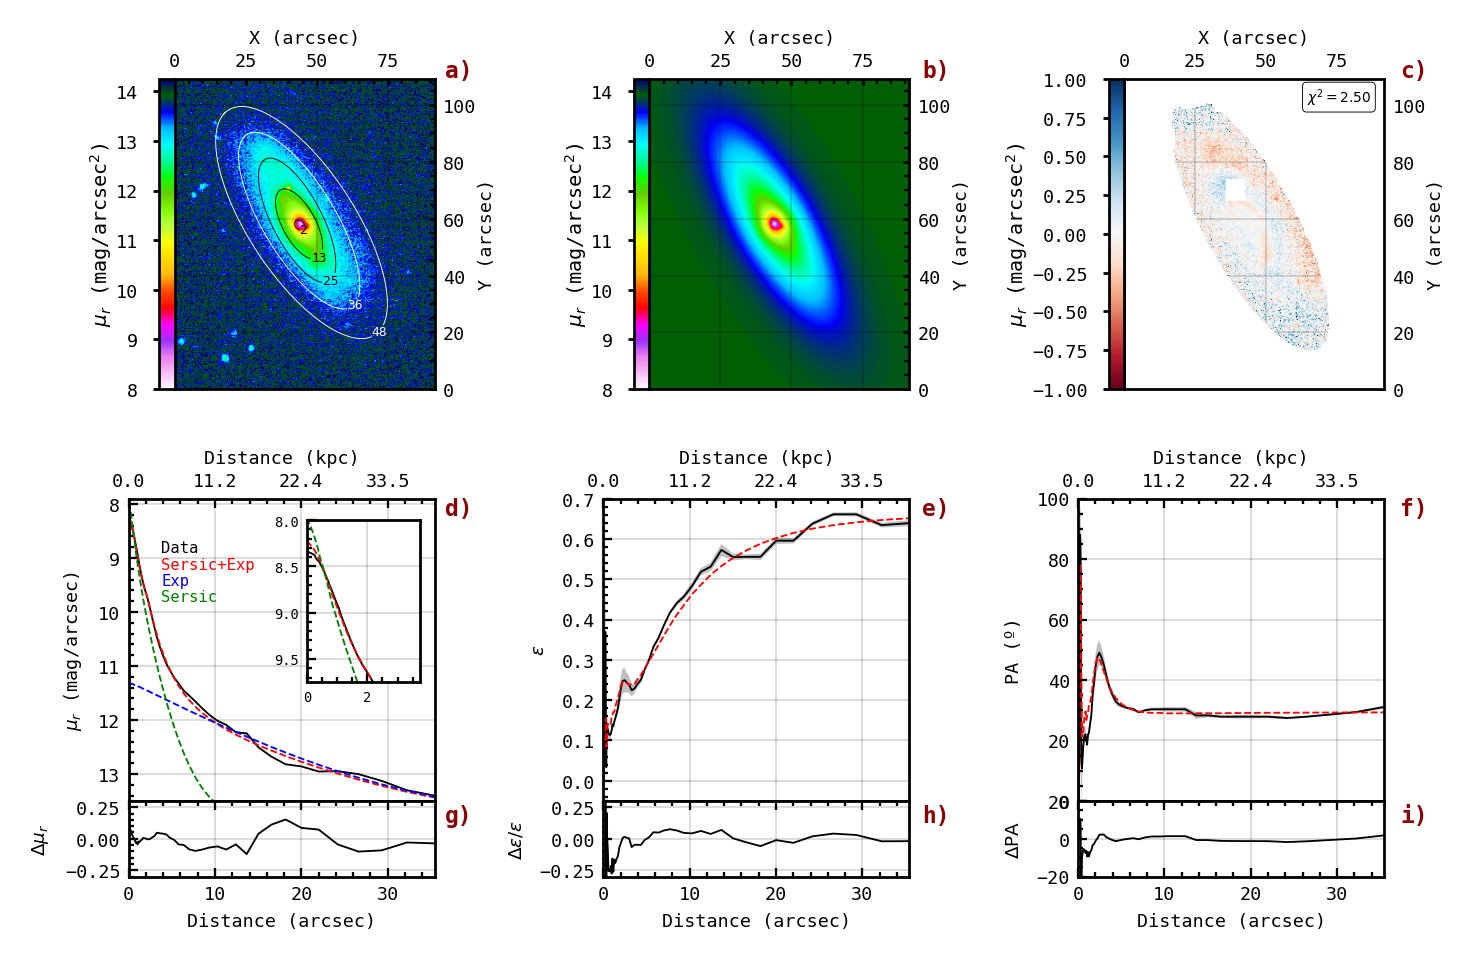
\includegraphics[width=\textwidth]{images/fit_sersic_exp_and_sersic_bump.png}
  \caption{Photometric fitting of UGC09629 incorporating an exponential and a Sérsic model for the galaxy and an additional Sérsic model for the luminous bulb near the center of the galaxy, supplemented with elliptical isophote profile analysis. The reduced $\chi^2$ for the overall fit was 2.50. Image description is the same as Figure 2 in the main text.}
  \label{fig:your_label}
\end{figure*}


\begin{figure*}[h!]
\renewcommand{\thefigure}{S2}
  \centering
  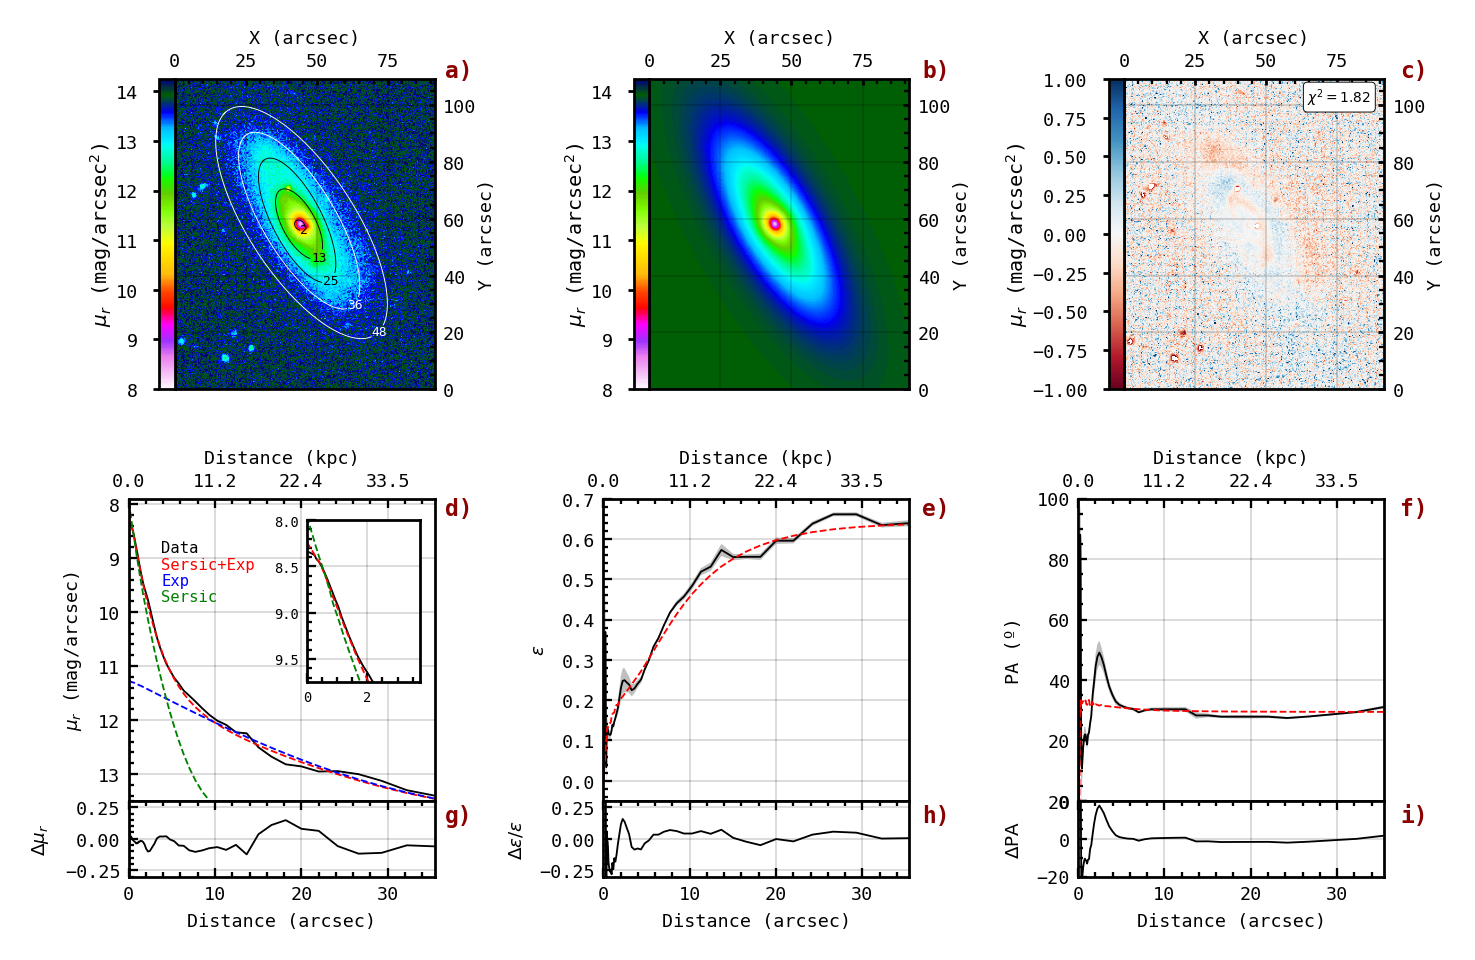
\includegraphics[width=\textwidth]{images/fit_sersic_exp_own_mask.png}
  \caption{Photometric fitting of UGC09629 incorporating an exponential and a Sérsic model for the galaxy and using a customized \textit{ad hoc} mask, supplemented with elliptical isophote profile analysis. The reduced $\chi^2$ for the overall fit was 1.82. Image description is the same as Figure 2 in the main text.}
  \label{fig:your_label}
\end{figure*}
